%% LaTeX-Beamer template for KIT design
%% by Erik Burger, Christian Hammer
%% title picture by Klaus Krogmann
%%
%% version 2.1
%%
%% mostly compatible to KIT corporate design v2.0
%% http://intranet.kit.edu/gestaltungsrichtlinien.php
%%
%% Problems, bugs and comments to
%% burger@kit.edu

% Diese Zeile für Upload-Datei benutzen (sonst auskommentieren)
\documentclass[handout]{beamer}

% Diese Zeile für Präsentation benutzen (sonst auskommentieren)
%\documentclass[18pt]{beamer}

%Load Preconfig
%% LaTeX-Beamer template for KIT design
%% by Erik Burger, Christian Hammer
%% edited by Cihat Gündüz, Peter Wolf
%%
%% version 3.0
%%
%% mostly compatible to KIT corporate design v2.0
%% http://intranet.kit.edu/gestaltungsrichtlinien.php
%%
%% Problems, bugs and comments to
%% burger@kit.edu

% Selbstdefinierte Kommandos als Arbeitsbeschleunigung:
\newcommand{\f}[1]{\textbf{#1}}					% nutzen in der Form: \f{FETTER TEXT}
\newcommand{\p}{\pause}						% nutzen in der Form: \p (statt \pause}
\newcommand{\code}[1]{\lstinputlisting[caption=#1]}		% Nutzen in der Form: \code{TITEL}{QUELLE}
\newcommand{\cd}[1]{\lstinline[basicstyle=\normalsize\ttfamily]{#1}}		% Nutzen in der Form: \cd{KURZER QUELLTEXT}
\newcommand{\scd}[1]{\lstinline[basicstyle=\scriptsize\ttfamily]{#1}}	% Nutzen in Form: \scd{KLEINER QUELLTEXT} 	% scd steht für Small CoDe
\newcommand{\mcd}[1]{\lstinline[basicstyle=\footnotesize\ttfamily]{#1}}	% für mittlere Größe verwenden!
\newcommand{\bcode}[1]{\lstinputlisting[caption=#1,basicstyle=\normalsize\ttfamily]}	% Big Code, Nutzen in der Form: \bcode{TITEL}{QUELLE}
\newcommand{\scode}[1]{\lstinputlisting[caption=#1,basicstyle=\tiny\ttfamily]} 	%Small Code, Nutzen in der Form: \scode{TITEL}{QUELLE}


%% SLIDE FORMAT

% use 'beamerthemekit' for standard 4:3 ratio
% for widescreen slides (16:9), use 'beamerthemekitwide

\usepackage{templates/beamerthemekit}
% \usepackage{templates/beamerthemekitwide}

% Erlaube Code-Integration mit listings
\definecolor{kit-gray}{RGB}{224,224,224}
\definecolor{kit-green}{RGB}{32,149,128}
\usepackage{listings}
\usepackage{courier}
\usepackage{animate}
\lstset{
         language=Java,
         basicstyle=\scriptsize\ttfamily, % Sktipgröße und Standardschrift
         numbers=left,              	% Ort der Zeilennummern
         numberstyle=\tiny,         	% Stil der Zeilennummern
         %stepnumber=2,               	% Abstand zwischen den Zeilennummern
         numbersep=5pt,              	% Abstand der Nummern zum Text
         tabsize=2,                  		% Größe von Tabs
         extendedchars=true,         %
         breaklines=true,            	% Zeilen werden umgebrochen
         %keywordstyle=\color{red},
    	frame=t,         
	%frameround=tftf, 
         keywordstyle=[1]\textbf,    	% Stil der Keywords
         stringstyle=\color{blue}\ttfamily, 	% Farbe der String
         showspaces=false,           	% Leerzeichen anzeigen?
         showtabs=false,             	% Tabs anzeigen?
         xleftmargin=17pt,
         framexleftmargin=17pt,
         framexrightmargin=6pt,
         framexbottommargin=4pt,
         backgroundcolor=\color{kit-gray},
         commentstyle=\color{kit-green},
         showstringspaces=false    	% Leerzeichen in Strings anzeigen?       
         %numberbychapter=false 
 }

\usepackage{caption}
\DeclareCaptionFont{white}{\color{white}}
\DeclareCaptionFormat{listing}{\colorbox[cmyk]{0.79, 0.18, 0.57,0.03}{\parbox{\textwidth}{\hspace{4pt}#1#2#3}}}
\captionsetup[lstlisting]{format=listing,labelfont=white,textfont=white, singlelinecheck=false, margin=0pt, font={bf,footnotesize}}


%% TITLE PICTURE

% if a custom picture is to be used on the title page, copy it into the 'logos'
% directory, in the line below, replace 'mypicture' with the 
% filename (without extension) and uncomment the following line
% (picture proportions: 63 : 20 for standard, 169 : 40 for wide
% *.eps format if you use latex+dvips+ps2pdf, 
% *.jpg/*.png/*.pdf if you use pdflatex)

\titleimage{KIT-Titel}

% DEUTSCHE SPRACHE EINBINDEN
\usepackage[utf8]{inputenc}

% Deutsche Ausgabe anpassen
\usepackage[T1]{fontenc}

% Für korrekte Unterstreichung etc.
\usepackage[normalem]{ulem}

% Navigationssymbole unten abschalten
\beamertemplatenavigationsymbolsempty

%% TikZ INTEGRATION

% use these packages for PCM symbols and UML classes
% \usepackage{templates/tikzkit}
% \usepackage{templates/tikzuml}


\definecolor{dgreen}{HTML}{006600}
\definecolor{dyellow}{HTML}{FFCC00}

% the presentation starts here
%------------------------------------------------------------------------------------------------

\title[Hardwareimplementierungen künstlicher neuronaler Netze]{Proseminar: Hardwareimplementierungen künstlicher neuronaler Netze}
\author{Leon Jungemeyer}
\date{24.01.2020}

\institute{Professur für Rechnerarchitektur und Parallelverarbeitung}

% Bibliography

\usepackage[citestyle=authoryear,bibstyle=numeric,hyperref,backend=biber]{biblatex}
\usepackage{graphicx}
\usepackage{blindtext}
\addbibresource{templates/example.bib}
\bibhang1em

\begin{document}

    % change the following line to "ngerman" for German style date and logos
    \selectlanguage{ngerman}

    %title page
    \begin{frame}
        \titlepage
    \end{frame}

    %%%%%%%%%%%%%%%%%%%%%%%%%%%%%%%%%%%%%%%%%%%%%%%%%%%%%%%%%%%%%%%%%%%%%%%%%%%%%%%%%%%%%%%%%%%%%%
    \section{Einleitung}

    \begin{frame} {Was ist ein ANN? - Neuronen}
        \begin{center}
            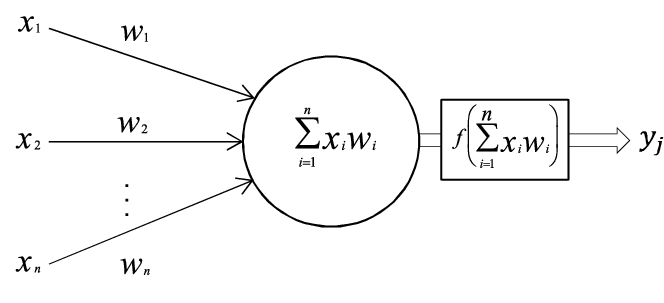
\includegraphics[width=290px]{resources/ann-neuron.png} \\
            \tiny Using deep learning to investigate the neuroimaging correlates of psychiatric and neurological disorders: Methods and applications - Scientific Figure on ResearchGate.
            \tiny Available from: \href{https://www.researchgate.net/figure/a-The-building-block-of-deep-neural-networks-artificial-neuron-or-node-Each-input-x\_fig1\_312205163}{https://www.researchgate.net/figure/a-The-building-block-of-deep-neural-networks-artificial-neuron-or-node-Each-input-x\_fig1\_312205163} \\
            \tiny [accessed 22 Jan, 2020]
        \end{center}
    \end{frame}

    \begin{frame} {Was ist ein ANN? - Synapsen}
        \begin{center}
            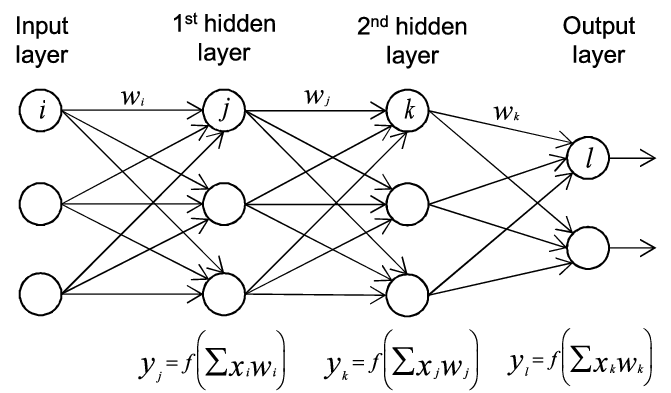
\includegraphics[width=290px]{resources/ann-neuron2.png} \\
            \tiny Using deep learning to investigate the neuroimaging correlates of psychiatric and neurological disorders: Methods and applications - Scientific Figure on ResearchGate.
            \tiny Available from: \href{https://www.researchgate.net/figure/a-The-building-block-of-deep-neural-networks-artificial-neuron-or-node-Each-input-x\_fig1\_312205163}{https://www.researchgate.net/figure/a-The-building-block-of-deep-neural-networks-artificial-neuron-or-node-Each-input-x\_fig1\_312205163} \\
            \tiny [accessed 22 Jan, 2020]
        \end{center}
    \end{frame}


    \begin{frame} {Aktivierungsfunktion}
        \begin{center}
            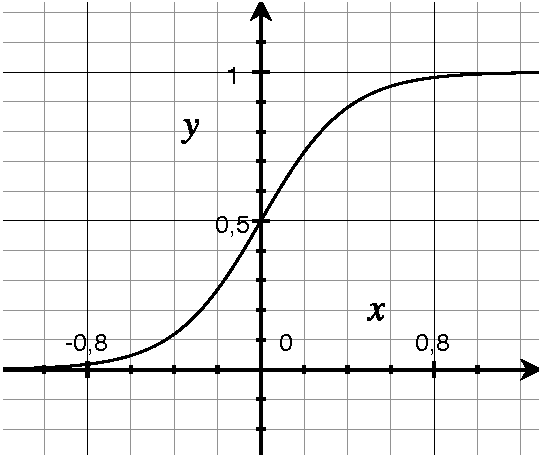
\includegraphics[width=220px]{../resources/sigmoid.pdf} \\
            \tiny Sigmoid activation function. $y = \frac{1}{1+e^{-5x}}$
        \end{center}
    \end{frame}

    \section{Neuronen}

    \subsection{Digitale Neuronen}

    \begin{frame}{Digitale Neuronen}
        \begin{itemize}[<+->]
            \item Eingabe/Ausgabe Digital
            \item Werte typischerweise floating Point
            \item Manchmal: Ganzzahlig
            \item Umsetzung in CMOS
        \end{itemize}
    \end{frame}

    \begin{frame}{Digitale Neuronen - Gewichte}
        \begin{itemize}[<+->]
            \item Verschiedene Arten von Gewichtsspeichern
            \begin{itemize}
                \item Shift-registern
                \item Flip-flops
                \item RAM
            \end{itemize}
            \item höhere Präzision -> mehr Speicher
            \item digitale Speicher leicht änderbar
        \end{itemize}
    \end{frame}

    \begin{frame}{Digitale Neuronen - Gewichtete Summe}
        \begin{itemize}[<+->]
            \item $x_i \times w_i$ für jede Synapse
            \item relativ aufwendige float-Operationen
            \item Summe kann zu Präzisionsverlust führen
            \item Hardware kann geteilt werden
        \end{itemize}
    \end{frame}

    \begin{frame}{Digitale Neuronen - Aktivierungsfunktion}
        \begin{itemize}[<+->]
            \item AF schwer zu berechnen
            \item Spezielle Hardware erforderlich
            \item Alternativ über look-up-table
            \begin{itemize}
                \item eventuell Präzisionsverlust
                \item kann zwischen Neuronen geteilt werden
            \end{itemize}
        \end{itemize}
    \end{frame}

    \subsection{Analoge Neuronen}

    \begin{frame}{Analoge Neuronen}
        \begin{itemize}[<+->]
            \item Eingabe/Ausgabe analog
            \item Werte Stromstärke oder Spannung
            \item Analoge Signalübertragung führt zu rauschen
            \item unterschiede in einer Baureihe
        \end{itemize}
    \end{frame}

    \begin{frame}{Analoge Neuronen - Gewichte}
        \begin{itemize}[<+->]
            \item Widerstand
            \begin{itemize}
                \item Wiederstände fest oder änderbar
                \item bei festem $R$: braucht von Werk trainiertes Netz
            \end{itemize}
            \item Digital
            \begin{itemize}
                \item Gewichte werden digital gespeichert
                \item bei bedarf in analoge $U$ konvertiert
                \item analoger speicher nicht Rauschanfällig
                \item Ergebnisse reproduzierbar
                \item leicht änderbar
                \item Quantisiert
            \end{itemize}
            \item Transistor
            \begin{itemize}
                \item Kondensator wird aufgeladen
                \item Transistor in bestimmten bereich linearer Widerstand
                \item Ladung ändern -> Widerstand ändern
                \item Ladung verfällt, muss erneuert werden
            \end{itemize}
        \end{itemize}
    \end{frame}

    \begin{frame}{Ananloge Neuronen - Gewichtete Summe}
        \begin{itemize}[<+->]
            \item Spannung: Spannungsaddierer, Reihenschaltung
            \item Strom: Parallelschalten
        \end{itemize}
    \end{frame}

    \begin{frame}{Analoge Neuronen - Aktivierungsfunktion}
        \begin{itemize}[<+->]
            \item lineare AF: ändern der Gewichte
            \item nichtlineare AF schwer zu berechnen
            \item Spezielle Hardware erforderlich
            \item z.B. Konvertierung nach Digital , LUT, Konvertierung nach Analog
            \item Je nach Hardware AF nicht änderbar
        \end{itemize}
    \end{frame}

    \begin{frame} {Analoge Neuronen}
        \begin{center}
            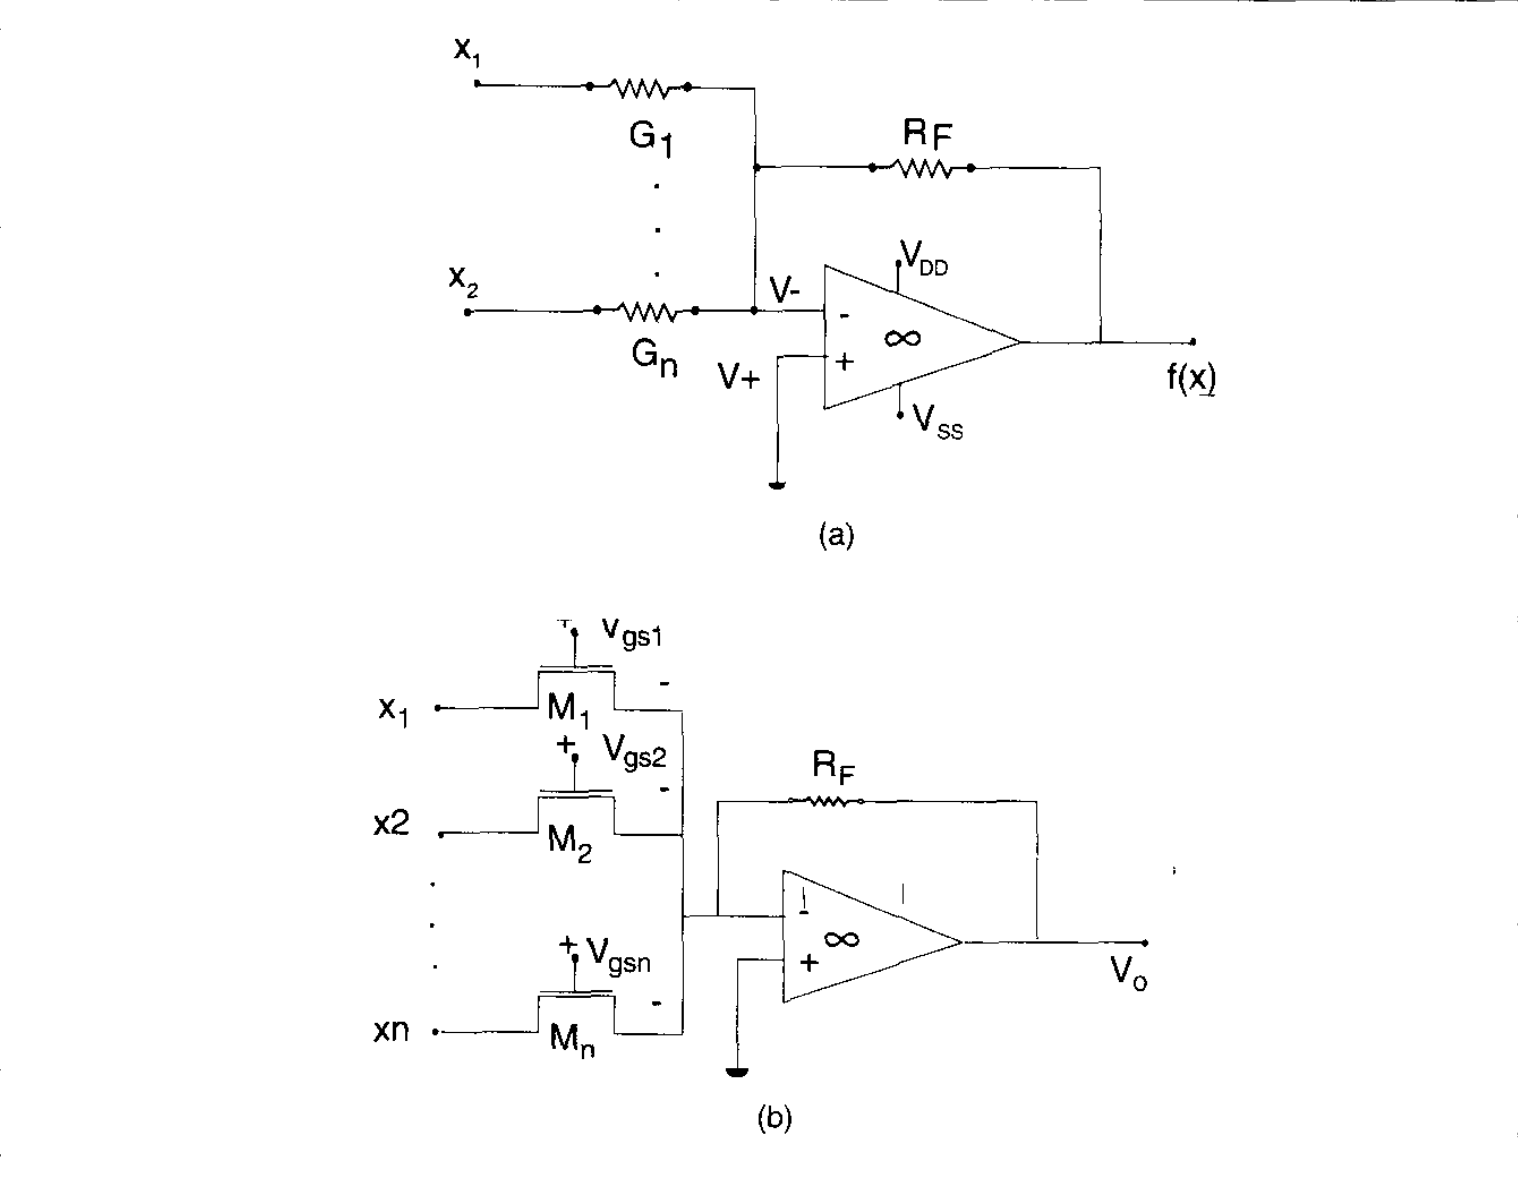
\includegraphics[width=220px]{../resources/analog-weights.png} \\
            \tiny Jacek M Zurada. Analog implementation of neural networks. IEEE
            Circuits and Devices Magazine, Fig. 1, 8(5):36–41, 1992.
        \end{center}
    \end{frame}

    \begin{frame} {Vergleich}
        \begin{itemize}
            \item Analoge Neuronen:
            \begin{itemize}
                \item höherer Energieverbrauch
                \item schneller
            \end{itemize}
            \item Digitale Neuronen:
            \begin{itemize}
                \item kein/weniger Rauschen
                \item einfachere Gewichtänderungen
            \end{itemize}
        \end{itemize}
    \end{frame}

    \section{Neurochips}

    \begin{frame} {Neurochips}
        \begin{itemize}
            \item Zusammengesetzt aus vielen Neuronen
            \item Typischerweise in Schichten(Layern)
            \item Schichten müssen nicht voll verbunden sein
        \end{itemize}
    \end{frame}

    \subsection{Digitale Neurochips}
    \begin{frame} {Digitale Neurochips}
        \begin{itemize}
            \item Slice Architecture
            \begin{itemize}
                \item Blöcke zum Aufbau eines NN
                \item Ähnlich zu grafischem NN
                \item Jedes Neuron berechnet und gibt weiter
                \item Neuronen wissen nichts über Rest des Netzes
            \end{itemize}
        \end{itemize}
    \end{frame}

    \begin{frame} {Digitale Neurochips}
        \begin{itemize}
            \item Systolic array
            \begin{itemize}
                \item Viele Parallelprozessoren
                \item Jeder Prozessor jenau für eine Operation zuständig
                \item Ergebnisse werden weiter gegeben
                \item Gewichte typischerweise extern Gespeichert
                \item AF normal vie LUT
            \end{itemize}
        \end{itemize}
    \end{frame}

    \subsection{Analoge Neurochips}

    \begin{frame} {Analoge Neurochips}
        \begin{itemize}
            \item Je mehr Neuronen/Synapsen desto komplexer
            \item Analoge Gewichtsspeicher müssen kontinuierlich aktualisiert werden
            \item Digitale Gewichtsspeicher haben begrenzte Write Cycles
            \item Interne Berechnungen sehr schnell
            \begin{itemize}
                \item nicht an Clock cycles gebunden
                \item elektronische Effekte müssen beachtet werden
            \end{itemize}
            \item Rauschen kann sich durch gesamtes Netz fortsetzen
            \item Ungenauigkeiten können Klassifikationsgenauigkeit beeinflussen
        \end{itemize}
    \end{frame}

    \subsection{Hybride Neurochips}

    \begin{frame}{Hybride Neurochips}
        \begin{itemize}
            \item Kombinieren Vorteile von analog und digital
            \item I/O i.d.R. digital
            \item Interne Berechnungen analog
            \item Gewichte typischerweise digital gespeichert
            \item Dadurch lässt sich Rauschen reduzieren, Geschwindigkeit erhöhen
        \end{itemize}
    \end{frame}

    \begin{frame}{Vergleich}
        \begin{itemize}
            \item Gewichte bei digitalem Speicher quantisiert
            \begin{itemize}
                \item geringe Auswirkungen auf Genauigkeit
                \item wichtiger ist richtiges Runden
            \end{itemize}
            \item Analoge Ausgabe rauschbehaftet
            \item Ausgabe kann unter Rauschen leiden
            \item Analoge Gewichte schwer änderbar, on-chip learning schwer
            \item Analog schneller
        \end{itemize}
    \end{frame}

    \section{Lernen}

    \begin{frame}
        \begin{itemize}
            \item Algorithmen machen viele kleine Änderungen
            \item Schlecht für Gewichtsspeicher
            \item Manche Algorithmen brauchen wissen über Netzwerktopologie
            \item -> Extra Hardware zum Trainieren erforderlich
            \item viele Anwendungen kommen ohne on-chip learning aus
        \end{itemize}
    \end{frame}

    \section{Ausblick}

    \begin{frame}{Ausblick}
        \begin{itemize}
            \item Memristor hat wiederstand abhängig von durchflossener Ladung
            \item damit: anpassbarer Gewichstsspeicher
            \item zusätzlich: Gewichtsmultiplikation
            \item in Spiking Neuralnetworks: Lernen durch häufiges "feuern"
            \item -> kein wissen über Topologie nötig
        \end{itemize}
    \end{frame}

    \begin{frame}{Fazit}
        \begin{itemize}
            \item Hardware ANNs brauchen viel wissen über Netzwerk
            \item Nicht so universell wie "normale Prozessoren"
            \item lernen auch für Hardware ANNs sehr komplex
            \item In Realität GPUs zur Beschleunigung verwendet
        \end{itemize}
    \end{frame}

    %%%%%%%%%%%%%%%%%%%%%%%%%%%%%%%%%%%%%%%%%%%%%%%%%%%%%%%%%%%%%%%%%%%%%%%%%%%%%%%%%%%%%%%%%%%%%%

    \section{Diverses}

\end{document}
